%% This is file `elsarticle-template-1-num.tex',
%%
%% Copyright 2009 Elsevier Ltd
%%
%% This file is part of the 'Elsarticle Bundle'.
%% ---------------------------------------------
%%
%% It may be distributed under the conditions of the LaTeX Project Public
%% License, either version 1.2 of this license or (at your option) any
%% later version.  The latest version of this license is in
%%    http://www.latex-project.org/lppl.txt
%% and version 1.2 or later is part of all distributions of LaTeX
%% version 1999/12/01 or later.
%%
%% The list of all files belonging to the 'Elsarticle Bundle' is
%% given in the file `manifest.txt'.
%%
%% Template article for Elsevier's document class `elsarticle'
%% with numbered style bibliographic references
%%
%% $Id: elsarticle-template-1-num.tex 149 2009-10-08 05:01:15Z rishi $
%% $URL: http://lenova.river-valley.com/svn/elsbst/trunk/elsarticle-template-1-num.tex $
%%
\documentclass[preprint,12pt]{elsarticle}

%% Use the option review to obtain double line spacing
%% \documentclass[preprint,review,12pt]{elsarticle}

%% Use the options 1p,twocolumn; 3p; 3p,twocolumn; 5p; or 5p,twocolumn
%% for a journal layout:
%% \documentclass[final,1p,times]{elsarticle}
%% \documentclass[final,1p,times,twocolumn]{elsarticle}
%% \documentclass[final,3p,times]{elsarticle}
%% \documentclass[final,3p,times,twocolumn]{elsarticle}
%% \documentclass[final,5p,times]{elsarticle}
%% \documentclass[final,5p,times,twocolumn]{elsarticle}

%% if you use PostScript figures in your article
%% use the graphics package for simple commands
%% \usepackage{graphics}
%% or use the graphicx package for more complicated commands
\usepackage{graphicx}
%% or use the epsfig package if you prefer to use the old commands
%% \usepackage{epsfig}

\usepackage[utf8]{inputenc}		% Codificacao do documento (conversão automática dos acentos)
\usepackage{hyperref}


%% The amssymb package provides various useful mathematical symbols
\usepackage{amssymb}
%% The amsthm package provides extended theorem environments
%% \usepackage{amsthm}

%% The lineno packages adds line numbers. Start line numbering with
%% \begin{linenumbers}, end it with \end{linenumbers}. Or switch it on
%% for the whole article with \linenumbers after \end{frontmatter}.
%% \usepackage{lineno}

%% natbib.sty is loaded by default. However, natbib options can be
%% provided with \biboptions{...} command. Following options are
%% valid:

%%   round  -  round parentheses are used (default)
%%   square -  square brackets are used   [option]
%%   curly  -  curly braces are used      {option}
%%   angle  -  angle brackets are used    <option>
%%   semicolon  -  multiple citations separated by semi-colon
%%   colon  - same as semicolon, an earlier confusion
%%   comma  -  separated by comma
%%   numbers-  selects numerical citations
%%   super  -  numerical citations as superscripts
%%   sort   -  sorts multiple citations according to order in ref. list
%%   sort&compress   -  like sort, but also compresses numerical citations
%%   compress - compresses without sorting
%%
%% \biboptions{comma,round}

% \biboptions{}


%% \journal{Journal Name}

\begin{document}

\begin{frontmatter}

%% Title, authors and addresses

%% use the tnoteref command within \title for footnotes;
%% use the tnotetext command for the associated footnote;
%% use the fnref command within \author or \address for footnotes;
%% use the fntext command for the associated footnote;
%% use the corref command within \author for corresponding author footnotes;
%% use the cortext command for the associated footnote;
%% use the ead command for the email address,
%% and the form \ead[url] for the home page:
%%
%% \title{Title\tnoteref{label1}}
%% \tnotetext[label1]{}
%% \author{Name\corref{cor1}\fnref{label2}}
%% \ead{email address}
%% \ead[url]{home page}
%% \fntext[label2]{}
%% \cortext[cor1]{}
%% \address{Address\fnref{label3}}
%% \fntext[label3]{}

\title{Experimento 01 - Comparação entre algoritmos de busca/otimização de hiper-parâmetros}

%% use optional labels to link authors explicitly to addresses:
%% \author[label1,label2]{<author name>}
%% \address[label1]{<address>}
%% \address[label2]{<address>}

\author{Augusto César Benvenuto de Almeida}

\begin{abstract}

Neste experimento foi realizado uma comparação entre diversas técnicas de busca de hiper-parâmetros, entre elas podemos destacar o Particle Swarm Optimization (PSO) e o Covariance Matrix Adaptation Evolution Strategy (CMA-ES). Analisando os dados coletados e aplicando testes estatísticos não-paramétricos é possível perceber que existem claras diferenças entre o desempenho dos algoritmos. Entre os testados, os que apresentaram melhor desempenho foi o PSO, Random Search e Grid Search. Porém o PSO conseguiu sempre ser o mais rápido dentre os métodos testados.

\end{abstract}


\end{frontmatter}

%%
%% Start line numbering here if you want
%%
%% \linenumbers

%% main text
\section{Motivação}
\label{S:1}

Como o espaço de busca dos parâmetros para cada técnica de Machine Learning costuma ser contínuo e de alta dimensionalidade, para atingir os valores ótimos é necessário uma busca exaustiva de baixa granularidade, demandando assim um alto custo computacional.
Para resolver esse problema existem técnicas que servem para realizar essa busca de maneira a diminuir os custos de tempo e processamento.

\section{Objetivo}

Este experimento tem como objetivo verificar quais das funções disponíveis atingem o melhor resultado dentre as séries de retorno das ações componentes do índice IBOVESPA.

As técnicas a serem comparadas serão:

\subsection{Random Search (RS)}

Random Search é a técnica mais simples de todos os algoritmos testados, nela os parâmetros são gerados de forma aleatória seguindo uma distribuição uniforme num dado limite.

\subsection{Grid Search (GS)}

Grid Search é um método de busca não direcionado que consiste em testar um conjunto de valores pré-definidos para cada parâmetro. Uma grade é construída a partir do produto cartesiano desses conjuntos de valores.

Essa técnica também é bastante simples, porém permite que os parâmetros sejam gerados em diversas combinações diferentes.

\subsection{Particle Swarm Optimization (PSO)}

Particle Swarm Optimization \cite{Kennedy:2010} \cite{Clerc2002} (PSO) é um método heurístico de otimização, simula um conjunto de partículas que se movem no espaço de busca.

\subsection{Nelder-Mead (NM)}

Nelder-Mead \cite{Nelder1965} é um método numérico utilizado para encontrar os parâmetros que minimizam uma função objetivo em um espaço multi-dimensional.

Apresenta uma limitação pois precisa de um ponto inicial para iniciar a busca, o que pode levar a convergências de ótimos locais.

\subsection{Covariance Matrix Adaptation Evolution Strategy (CMA-ES)}

Covariance Matrix Adaptation Evolutionary Strategy \cite{Hansen2001} \cite{wiki:xxx} é um algoritmo evolucionário para otimização de funções contínuas, ele consegue se adaptar dinamicamente ao espaço de busca, permitindo assim buscas eficientes.

\section{Metodologia}

Primeiro passo para realizar o experimento foi conseguir a base de dados, para tal foi utilizado o sistema do Yahoo! Finance \cite{yahoo} para conseguir as séries do IBOVESPA ( 43 dos 70 componentes do índice). 

Os dados adquiridos apresentam dados temporais e diversos dados financeiros, será utilizado e avaliado no experimento e tese apenas a série de preços ajustados de fechamento, ajustes necessários para equalizar o preço no tempo devido a ações de desdobramento ou grupamento \cite{invest}.

Vale notar que os dados utilizados apresentam apenas valores colhidos nas quartas-feiras, isso foi feito para evitar um efeito\cite[p. 404]{mptbook} conhecido no mercado no início e fim de semana.

Com as séries em mãos é necessário realizar uma transformação nos dados para conseguir a série de retornos, a operação aplicada é:

\begin{equation}
r_{t} = \frac{p_{t} - p_{t-1}}{p_{t-1}}
\end{equation}

Após calculada, precisamos ainda criar a matriz contendo os padrões de entrada e saídas para os algoritmos de Machine Learning, nessa fase é necessário um parâmetro $p$ extra responsável pela dimensão do problema, nesse caso é a quantidade de lags usados para prever o próximo valor.


\begin{figure}[h]
	\centering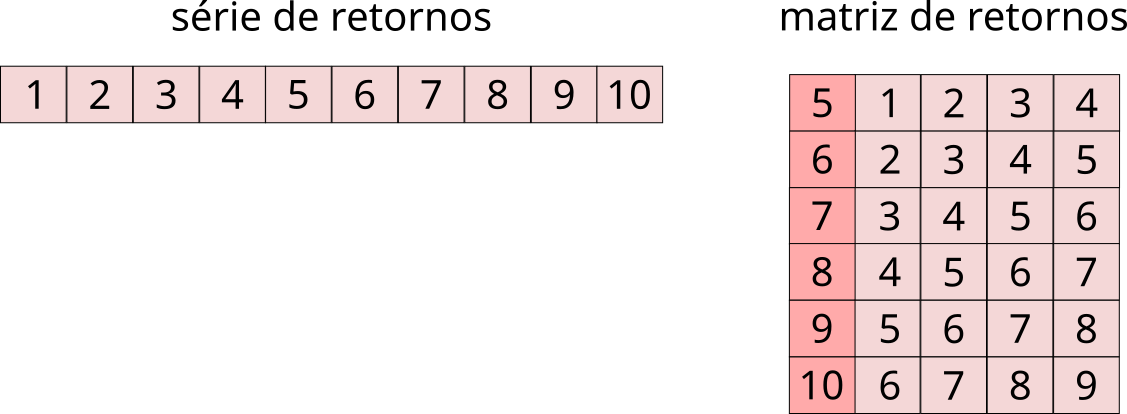
\includegraphics[width=0.8\linewidth]{g4145}
	\caption{Exemplo de matriz gerada com parâmetro $p$ = 4, valor de saída na primeira coluna e de entrada nas demais.}
\end{figure}


Para conseguir alguma relevância estatística serão feitas 50 execuções de um cross-validation (CV) proposto por Hyndman \cite{hyndman} para cada algoritmo de busca, a variável a ser analisada será o valor da raiz quadrada do erro médio quadrático (RMSE) resultante de cada  de cada CV.

Para exemplificar, imagine que a matriz de retornos seja dividida em k-folds (5, por exemplo) sem que haja permutação dos padrões para que não ocorra perda de informação de autocorrelação entre os dados, consequência inerente das séries temporais. 

Então acontecerão 4 processos de treinamento/teste de forma sequencial, no primeiro passo usa-se o fold-1 para treinamento do regressor e o fold-2 para teste, é então calculado o RMSE do conjunto de teste e seu resultado é salvo. No próximo passo o fold-2 é agregado ao anterior e ambos são usados como treinamento para testar o fold-3, e assim por diante. Desse jeito é possível representar o comportamento temporal no cross-validation e se aproximar do que ocorre no mundo real. O resultado final do CV é exatamente a média dos RMSEs calculados nessa etapa.

Exemplo:\\

1 : folds treinamento [1], fold teste [2]

2 : folds treinamento [1 2], fold teste [3] 

3 : folds treinamento [1 2 3], fold teste [4] 

4 : folds treinamento [1 2 3 4], fold teste [5] \\



Após a execução das 50 iterações para cada algoritmo de busca será gerada então uma matriz de 50 linhas e 5 colunas contendo todos os resultados obtidos, a primeira análise feita é se a distribuição dos valores de RMSE de cada técnica é igual, para tal foi usado um teste estatístico não-paramétrico, o \textbf{Kruskal-Wallis H-test}. Esse teste é o equivalente não-paramétrico do ANOVA e sua hipótese nula afirma que as distribuições dos grupos são iguais.

Se a hipótese for rejeitada é criada então uma matriz de 5 linhas e 5 colunas para verificar onde estão as diferenças entre os algoritmos, cada elemento da matriz é o resultado de um teste não-paramétrico entre os pares de técnicas \textit{i} e \textit{j}, o teste é o mesmo realizado anteriormente, porém quando o número de grupos é 2 (teste pareado) ele é conhecido por \textbf{Mann–Whitney U test}, equivalente não paramétrico do t-test.

Exemplo:


\begin{table}[h]
	\centering
	\begin{tabular}{|r|r|r|r|r|r|}
		\hline
		& rs & gs & pso & nm & cma-es \\
		\hline
		rs & 0 &   0 &   1 &   0 &   1 \\
		\hline
		gs & 1 &     0 &     1 &     0 &     1 \\
		\hline		
		pso & 0 &     0 &     0 &     0 &     0 \\
		\hline		
		nm & 1 &     1 &     1 &     0 &     1 \\
		\hline		
		cma-es & 0 &     0 &     0 &     0 &     0 \\
		\hline
	\end{tabular}
	\caption{Matriz contendo o resultado dos testes pareados}
\end{table}




Se a matriz for criada, ou seja, existe diferença estatística entre os algoritmos, é calculado um vetor com a soma de cada linha da matriz para criar um ranking dessa técnica em relação as outras. 

A matriz é formada por 0's e 1's, onde uma linha representa o desempenho de uma técnica em relação as outras, se for 0 temos a possibilidade de que as técnicas não apresentam diferença estatística entre si ou então o i-ésimo algoritmo é melhor que o j-ésimo ( apresenta um RMSE médio menor, nesse caso melhor pois tratamos de erro ), se for 1 só existe a possibilidade que existe diferença estatística entre as técnicas e que a i-ésima apresenta um pior desempenho ( RMSE médio maior ).

Então cada elemento do vetor varia entre 0 e 4, onde o primeiro representa que aquele algoritmo não foi pior que nenhum outro e 4 indica que ele foi pior que todos os outros.

Esse experimento foi feito utilizando 3 diferentes regressores, para verificar se os resultados eram consistentes entre diferentes técnicas de Machine Learning, foram escolhidos o \textbf{elmK} \cite{GuangBinHuang2012}, \textbf{elmR} \cite{GuangBinHuang2012} e \textbf{svr} \cite{drucker1997support}.


\section{Resultados}

Nesta seção serão apresentados os resultados finais colhidos após processar 43 séries componentes do IBOVESPA nos 3 regressores propostos.


\subsection{elmK}



\begin{table}[h]
	\centering
	\begin{tabular}{lr}
		\hline
		Search Function   &   Ranking Sums \\
		\hline
		random search     &             39 \\
		grid search       &             49 \\
		particle swarm    &             27 \\
		nelder-mead       &            163 \\
		cma-es            &             97 \\
		\hline
	\end{tabular}
	\caption{Soma dos rankings encontrados para as 43 séries}
\end{table}

O resultado do \textit{elmK} mostra que o algoritmo que apresentou melhor desempenho foi o PSO, com o Random Search e Grid Search em seguida, respectivamente.

Além disso é feita mais uma checagem para dar uma força estatística ao resultado, é criada uma matriz contendo o vetor de rankings de cada uma das séries verificadas, formando assim uma matriz de 43 linhas e 5 colunas. É feito um teste não-paramétrico para verificar se os rankings dos algoritmos apresentam uma mesma distribuição.

\begin{table}[h]
	\centering
	\begin{tabular}{l r}
		
		Rankings have same distribution  &  False \\
		
	\end{tabular}
	\caption{Resultado do teste não-paramétrico descrito acima}
\end{table}

A hipótese nula foi negada, então é criada uma matriz quadrada contendo os resultados dos testes não-paramétricos pareados. A partir dela, gera-se um vetor final contendo o ranking definitivo.

Com isso temos o resultado final:


\begin{table}[h]
	\centering
	\begin{tabular}{lrrrr}
		\hline
		Search Function   &   Rank &   Rank Mean &      Time Mean \\
		\hline
		particle swarm    &      0 &    0.6279 &       1.6810  \\
		random search     &      0 &    0.9069 &       1.7933  \\
		grid search       &      1 &    1.1395  &       1.8438  \\
		cma-es            &      3 &    2.2558  &      1.6764  \\
		nelder-mead       &      4 &    3.7907   &     0.1941 \\
		\hline
	\end{tabular}
	
	\caption{Análise final para o \textit{elmK}}
\end{table}

O PSO e Random Search apresentaram os melhores resultados, apesar de não existir uma diferença estatística entre os dois, o primeiro conseguiu uma menor média nos rankings e um menor tempo médio de execução.


\subsection{elmR}

\begin{table}[h]
	\centering
	\begin{tabular}{lr}
		\hline
		Search Function   &   Ranking Sums \\
		\hline
		random search     &             76 \\
		grid search       &             17 \\
		particle swarm    &             40 \\
		nelder-mead       &            172 \\
		cma-es            &             63 \\
		\hline
	\end{tabular}
	
	\caption{Soma dos rankings encontrados para as 43 séries}
\end{table}

O resultado mostra que o algoritmo que apresentou melhor desempenho foi o GS, com o PSO e CMA-ES em seguida, respectivamente. Realizando mais uma vez um teste para verificar se os rankings apresentam uma mesma distribuição temos:

\begin{table}[h]
	\centering
	\begin{tabular}{l r}
		
		Rankings have same distribution  &  False \\
		
	\end{tabular}
	\caption{Resultado do teste não-paramétrico entre os rankings}
\end{table}

A hipótese nula foi negada, com isso temos o resultado final:

\begin{table}[h]
	\centering
	\begin{tabular}{lrrrr}
		\hline
		Search Function   &   Rank &   Rank Mean &      Time Mean \\
		\hline
		grid search       &      0 &    0.3953 &     3.8715  \\
		particle swarm    &      1 &    0.9302 &      3.4902  \\
		cma-es            &      2 &    1.4651  &     3.6026  \\
		random search     &      2 &    1.7674  &     3.8385  \\
		nelder-mead       &      4 &    4.0000    &    0.4778 \\
		\hline
	\end{tabular}
	
	\caption{Table caption}
\end{table}

O GS apresentou o melhor resultado, em seguida vem o PSO. Esse resultado pode ser entendido pelo fato de no \textit{elmR} o espaço de busca ser menor, apenas 1 dimensão do parâmetro de regularização $C$, pois o número de neurônios está fixo em 500. Isso deve ajudar um pouco o grid search, deixando a sua busca bem mais refinada do que o PSO. Mas apesar disso o PSO ainda conseguiu ser mais rápido.

\subsection{svr}

\begin{table}[h]
	\centering
	\begin{tabular}{lr}
		\hline
		Search Function   &   Ranking Sums \\
		\hline
		random search     &             18 \\
		grid search       &             10 \\
		particle swarm    &             30 \\
		nelder-mead       &            128 \\
		cma-es            &             89 \\
		\hline
	\end{tabular}
	
	\caption{Soma dos rankings encontrados para 34 séries}
\end{table}

O resultado mostra que o algoritmo que apresentou melhor desempenho foi o GS, com o RS e PSO em seguida, respectivamente. Realizando mais uma vez um teste para verificar se os rankings apresentam uma mesma distribuição temos:

\begin{table}[h]
	\centering
	\begin{tabular}{l r}
		
		Rankings have same distribution  &  False \\
		
	\end{tabular}
	\caption{Resultado do teste não-paramétrico entre os rankings}
\end{table}

A hipótese nula foi negada, com isso temos o resultado final:\\ \\

\begin{table}[h]
	\centering
	\begin{tabular}{lrrrr}
		\hline
		Search Function   &   Rank &   Rank Mean &     Time Mean \\
		\hline
		grid search       &      0 &    0.2941 &       38.9919   \\
		random search     &      0 &    0.5294 &         5.7148   \\
		particle swarm    &      1 &    0.8823 &         2.7880  \\
		cma-es            &      3 &    2.6176  &   0.2987 \\
		nelder-mead       &      4 &    3.7647  &        0.1305 \\
		\hline
	\end{tabular}
	
	
	\caption{Table caption}
\end{table}

Na terceira análise o PSO também fica em segundo lugar, atrás do Grid e Random Search, porém chega a ser 1 ordem de grandeza mais rápido. Isso deve ocorrer pois o \textit{svr} precisa resolver um problema de otimização para conseguir seus vetores de suporte, assim o GS deve entrar em áreas onde os parâmetros pedidos são muito difíceis e de convergência demorada.


\section{Conclusão}

Fazendo uma análise mais simplificada somando os rankings dos resultados finais temos que o GS tem 1 ponto, enquanto que o RS e PSO atingem 2 pontos, porém o PSO sempre consegue ser o mais rápido, num ambiente dinâmico e de alta frequência como da previsão de séries temporais, talvez seja melhor optar pela velocidade e pegar um método \textit{bom}, quase ótimo.

Todos os códigos, base de dados, resultados e documentos desse experimento estão disponíveis em \url{http://www.sharelatex.com}


\bibliographystyle{model1-num-names}
\bibliography{sample.bib}

\end{document}